% Chapter 2

\chapter{Social Media and Real-life Events} % Main chapter title

\label{events} % For referencing the chapter elsewhere, use \ref{Chapter1} 

\lhead{Chapter 2. \emph{Social Media and Real-life Events}} % This is for the header on each page - perhaps a shortened title
\doublespacing
\setlength{\parindent}{1cm}
\section{Social Media}
Social media is defined as a group of Internet-based applications that build on the ideological and technological foundations of Web 2.0, and that allow the creation and exchange of user-generated content \cite{kaplan2010users}. These Internet-based applications broadly ranges from blogs, microblogs, media sharing webistes, social bookmarking websites, social news to social networking websites. Brief descriptions of most popular types of social media websites is given below.

\subsection{Blogs}
A blog can be defined as a website that displays, in a reverse chronological order, the entries by one or more individuals and usually has links to comments on specific postings. Blogs often provide opinions, commentaries, or news on a particular subject, such as food, politics, or local news. Some of them also function as personal online diaries. Most of the time the entries of a blog is archived and is accessible at a later time. For the purpose of constant syndication, RSS or XML feeds for the blogs are made available. An individual entry in a blog is known as a blog post. A typical blog post can combine text, images and links to other blogs, web pages and other media related to its topic. The universe of all the blogs on the Internet is known as blogosphere \cite{agarwal2014time}.

\subsection{Microblogs}
Microblogs are similar to blogs, but a shorter version of it. Most of the microblogging websites pose limitations on the length of an individual post. Twitter\footnote{http://twitter.com}, one of the most popular microblogging website has a limitation of 140 characters. This makes the textual posts in these platforms, extremely concise. Users often associate URLs that lead to external sources of information related to the posts. A post may also contain attached image or video. The microblogging services mostly focus on short updates that are pushed out to anyone subscribed to receive the updates. This is made possible by enabling the users to form directed networks of \textit{friends} and \textit{followers}. The \textit{followers} of an user are entitled to get all the updates posted by him. Mostly these updates are public. 

\subsection{Media Sharing}
Media sharing services allow its users to upload and share various multimedia content such as pictures and videos. Most services have additional social features such as profiles, commenting, etc. The most popular are Instagram\footnote{http://instagram.com}, Pinterest\footnote{http://pinterest.com}, YouTube\footnote{http://youtube.com} and Flickr\footnote{http://flickr.com}. The media elements are often enriched with geographical and topical ``tags'' by the users who create them and the consumers who browse them. These tags acts as very useful meta data and allow automated programs to leverage them for efficient organization and retrieval of the videos and images that otherwise have very less textual content. 

\subsection{Social Bookmarking}
These are the genre of social media services that allow its users to save, organize and manage links to various websites and resources on the Internet. Most allow to ``tag" URLs for making them easy to search and share. The most popular are Delicious\footnote{http://delicious.com} and StumbleUpon\footnote{http://stumbleupon.com}. Some of the services like StumbleUpon also allow their users to form friendship networks. These websites often provide different browsing experiences through interfaces that help the users to search for most recent tags, most popular ones, and so on.

\subsection{Social News}
Social news websites allow people to post various news items or links to articles that are external to the website, and allow its users to cast their ``vote' on the items. The voting is the core social aspect as the items that get the most votes are displayed most prominently. This makes it an ideal crowdsourced news platform. It is up to the community of users to decide which news items gets seen by more people. Users can also ``tag'' the news stories and comment on them. The most popular are Digg\footnote{http://digg.com} and Reddit\footnote{http://reddit.com}.

\subsection{Social Networking}
Social networking websites are the ones that allow its users to connect with each other and form networks. The connections are generally non-directional and reciprocal. Two users who are connected to each other are considered as \textit{friends}. Usually the users in these webistes have a profile that presents the personal information of the user as provided by him. The users have various ways to interact with other users, and also sometimes have the ability to set up groups. These social networks may be based on a certain theme such as interests, location, and profession. Facebook\footnote{http://facebook.com} is the most popular personal social network and LinkedIn\footnote{http://linkedin.com} is the most popular professional network.

Some of the other types of websites that can also be categorized as social media services are, social messaging services, collaboration tools, rating or review sites, personal broadcasting tools, virtual worlds, and group buying. Table \ref{socialmediacat}, lists popular social media websites in different categories. Some of the websites may overlap and fall into multiple categories due to the broad range of services provided by them. For example, Facebook is not only a popular social networking website, but also a widely used social messaging service.

\begin{table}[h]
\centering
\caption{Popular social media websites belonging to different categories.}
\label{socialmediacat}
\begin{tabular}{|c|l|}
\hline
\textbf{Category} & \multicolumn{1}{c|}{\textbf{Popular Social Media Websites}} \\ \hline
\textbf{\textit{Blogs}} & Blogger, Medium, Wordpress, Squarespace \\ \hline
\textbf{\textit{Microblogs}} & Twitter, Tumblr, Posterous \\ \hline
\textbf{\textit{Media Sharing}} & \begin{tabular}[c]{@{}l@{}}Flickr, Instagram, YouTube, Vimeo, Dailymotion, Metacafe,\\ Viddler, Pinterest\end{tabular} \\ \hline
\textbf{\textit{Social Bookmarking}} & Delicious, StumbleUpon, Scoop, Slashdot \\ \hline
\textbf{\textit{Social News}} & Digg, Reddit, Newsvine, Propeller \\ \hline
\textbf{\textit{Social Networking}} & \begin{tabular}[c]{@{}l@{}}Facebook, Google Plus, LinkedIn, Ello, CafeMom,\\ Gather, Fitsugar\end{tabular} \\ \hline
\textbf{\textit{Virtual Worlds}} & Second Life, World of Warcraft, Farmville \\ \hline
\textbf{\textit{Group Buying}} & Groupon, Living Social, Crowdsavings \\ \hline
\textbf{\textit{Personal Broadcasting}} & Blog Talk radio, Ustream, Livestream \\ \hline
\textbf{\textit{Review/Rating}} & Amazon ratings, Angie’s List \\ \hline
\textbf{\textit{Collaboration Tools}} & Wikipedia, WikiTravel, WikiBooks \\ \hline
\textbf{\textit{Social Messaging}} & WhatsApp, Viber \\ \hline
\end{tabular}
\end{table}

According to Pew Research Center, Facebook, LinkedIn, Pinterest, Instagram and Twitter are the top five most popular social media websites used by American adult Internet users\footnote{http://www.pewinternet.org/2015/01/09/social-media-update-2014/}. The number of active users world-wide for all the five social media sites is shown in Table \ref{socialmediastat}. The numbers are obtained from the official pages of the respective websites. 

\begin{table}[h]
\centering
\caption{Number of active users for the top five social media websites used by American adults.}
\label{socialmediastat}
\begin{tabular}{|c|c|}
\hline
\textbf{Social Media Website} & \textbf{Number of Active Users} \\ \hline
\textbf{\textit{Facebook}} & 1.31 billion \\ \hline
\textbf{\textit{LinkedIn}} &  347 million \\ \hline
\textbf{\textit{Twitter}} & 289 million \\ \hline
\textbf{\textit{Instagram}} & 100 million \\ \hline
\textbf{Pinterest} & 70 million \\ \hline
\end{tabular}
\end{table}

\section{Characteristics of Social Media Websites\label{char}}
All the above social media websites exhibit certain common characteristics that is also responsible for their wide usage and huge popularity. We revisit some of the characteristics as already suggested by Agarwal et al. \cite{agarwal2010information} in the context of this dissertation.

\begin{enumerate}
\item \textbf{Accessibility:} Social media websites are freely available to whoever has an Internet connection. This makes these websites easily accessible all over the world. One of the latest initiatives by Facebook and Google is to make social media accessible even to the most remote corner of the world through their Internet.org\footnote{http://internet.org/} and ``Loon for All"\footnote{http://www.google.com/loon/} projects, respectively. With the popularity of hand held devices and increase in the Internet bandwidth, social media is accessible to anyone who has a smart phone and can use it. This is unlike the mainstream media or the print media, to which people subscribe and buy in the form of magazines, newspapers, journals, etc. Also, the mainstream media can be controlled by the government that may lead to propagation of biased information. For example, during the ``Egyptian Revolution of 2011", the mainstream media was biased, regulated by the government, and did not portray the true picture of the situation in Egypt. On the other hand, it was social media through which people discussed about the actual atrocities of the government and grouped together to incite the entire revolution \cite{hamdy2012framing}.

\item \textbf{Permanence:} Social media websites show dynamic nature and the content can be altered any time.  Users can easily edit the content shared by them. On the other hand the traditional print media and television media is not at all dynamic. Once an article is printed in a magazine/newspaper, or a television show is recorded and broadcasted, it cannot be changed.

\item \textbf{Reach:} As already presented in Table \ref{socialmediastat}, some of the popular social media websites have a reach of billions. Moreover, the ability of an individual user to simultaneously network with many other users makes this reach more effective than any other means of communication. These connections acts as networks of information flow, which helps in spreading any kind of information at a lightning speed \cite{bakshy2012role}. Also it provides equal opportunity to everyone for reaching their intended audience, unlike the traditional mainstream media. This characteristic is now regularly used by politicians for launching election campaigns and reaching out to people in social media \cite{metzgar2009social}. The marketers also leverage social media to a great extent. Event managers also take advantage of it, due to which social media has become an integral part of event management for getting connected with the event audience \cite{socialmediaforevents}. Social media is regularly used during planned events for making announcements, building and tracking audience, building focused communities, developing public relations \cite{eyrich2008pr}, and targeted marketing \cite{mangold2009social}. Due to easy reachability in social media, a focused group of people can also get together very quickly and organize events such as flash mobs and protest movements \cite{sen2012identifying}. 

\item \textbf{Recency:} The time lag at which communication can take place and information can flow is almost zero for the social media websites. Content is produced and communicated in real-time. Once this content is consumed, the users discuss about it instantaneously. Due to the reach and recency of social media it can make people aware of newsworthy events at a faster pace than traditional maintream media \cite{phelan2009using,petrovic2013can}. It might take hours, days, or sometimes months to present news or an event through mainstream media like newspapers, magazines and television. For example, the death of Bin Laden and the entire covert opertation was reported in Twitter even before the US president made an official announcement in the mainstream media \cite{ladendeathnews}. The users in social media were not only aware of the event but were also sharing and discussing it with great zeal.  Another example is of the theater shootings in Colorado \cite{coloradoshooting}. The shooting incident was reported, covered and analyzed in real-time, with traditional news media lagging behind social media by several minutes.

\item \textbf{Usability:} Social media sites are extremely easy to use and are user-friendly. An user does not require special training or skills to create content in a social media website. Whoever, can use a device connected to the Internet can share information in social media. Therefore, the operational cost of any social media application is mostly negligible. This is not the case for mainstream media. In order to report an event one needs to be skilled and specially trained. Also, the printing and telecasting of any event has to go through many other processes and has to be finally approved by the editor. This makes traditional media unusable by common people. The use of social media at the time of Internet blackout during the ``Egyptian Revolution of 2011" is a great example of its usability \cite{egyptianrevinternetblackout}. The Egyptian government had throttled the Internet connection and there was an Internet blackout for hours in order to stop the spreading of messages in social media, which was the major media of communication that led to the protest movements and finally to the revolution. In order to counterattack the government and to allow the Egyptians to use social media for giving latest updates, Google and Twitter launched a service that enabled them to leave a voicemail on a specific number. This voicemail was then posted in Twitter as a text message. Thus, people who didn't have a smart phone or didn't know how to use one could also post messages in social media.

%\item \textbf{Event-specific Information Content:} 

\end{enumerate}

%\section{Challenges in Social Media Mining}






%\subsection{Topic Detection and Tracking}
%
%\subsection{Automatic Content Extraction}
%
%\subsection{Multimedia Event Detection}

\section{Events in Social Media}



Events have been discussed from different perspectives and have gained attention in various areas of academics. Right from philosophy \cite{zalta2003stanford} to psychology \cite{zacks2001event} events have been defined in various ways. In the context of this dissertation we define events as defined by Becker et al. \cite{becker2011beyond}.

 

%The definition of event has received substantial attention across various academic areas, from philosophy (Zalta and Abramsky, 2003) to psychology (Zacks and Tversky,
%2001), over the years. An event is often defined as an abstract concept (Zalta and Abramsky, 2003), or with respect to its manifestation in a specific domain (e.g.,
%textual news \cite{allan2002topic}, video and audio clips (Westermann and Jain, 2007), social media \cite{becker2011beyond}.  In this
%dissertation, instead of providing yet another definition of an event, we define specific type of events in the context of Twitter (note that events on other social media
%platforms can be defined in a similar way), based on the traditional event definition (Troncy et al., 2010; Xie et al., 2008; Yang et al., 1998; Allan, 2002). We provide the
%following definitions:

\textbf{Event:} \textit{An event is defined as a real-world occurrence ($ E_{i}$) with an associated time period $T_{E_{i}}$ ($t^{start}_{E_{i}}$-$t^{end}_{E_{i}}$) and a time ordered stream of social media references $M_{E_{i}} = {\{m_{1_{E_{i}}},m_{2_{E_{i}}}, ... ,m_{n_{E_{i}}}, ... ,m_{z_{E_{i}}}\}}$, of substantial volume, discussing about the event and posted in time $T_{E_{i}}$}.

Although, this definition of event was originally proposed for the domain of Twitter, it can be applicable to all types of social media platforms as all of them fulfill the basic requirements of the above definition. Becker et al. \cite{becker2011beyond}, further categorizes events in social media into two categories, planned and unplanned, depending on whether the context of an event (e.g., topic or hashtags on Twitter, time, location) is available or not.



%Next, following the event categorization in (Becker et al., 2011), we classify the
%events in Twitter into two categories – planned events and unplanned events – depending on whether the context of an event (e.g., topic or hashtags on Twitter, time,
%location) is available to our toolbox.

\textbf{Planned event}: A planned event $PE_{i}$ is an event in Twitter with preknown corresponding event context information consisting both 
\begin{itemize}
\item topic or hashtags of the event.
\item time, at which $PE_{i}$ is planned to occur.
\end{itemize}

We only track planned events in this dissertation whose topics and hashtags are already known to us. For all the data collection efforts, an already known and event related popular hashtag is provided for bootstrapping the process of collecting event related messages. We consider all the messages in this stream as related to the event for which the query is placed and concentrate all our efforts to segregate high quality event-specific informative content from the non-informative ones. 


Next, in contrast to the planned event, there is no information about an unplanned event. To characterize and define such events, we have to rely on other signals that could indicate their presence. Such events are often known as trending events and is defined as follows for the domain of Twitter.

\textbf{Unplanned trending event}: An unplanned trending event is an event in Twitter with one or more features (e.g., terms) of the corresponding Twitter messages exhibiting bursty patterns during the event's time period.

We don't consider the trending events for this dissertation as don't intend to solve the task of identifying a trending event from streams of social media messages.



\section{Background: Entity Identity Information Management (EIIM) in Master Data Management}
The idea of Entity Identity Information Management (EIIM) as defined by Zhou et al. \cite{zhou2011entity}, is the collection and management of identity information of real-world entities with the goal of sustaining \textit{entity identity integrity}. \textit{Entity identity integrity} is one of the basic tenets of data quality that applies to the representation of a given domain of real-world entities in an information system \cite{talburt2011entity}. In order to maintain the property of \textit{entity identity integrity} following conditions should be satisfied:

\begin{enumerate}
\item Each real-world entity in the domain has one and only one representation in the information system.

\item Distinct real-world entities have distinct representations in the information system.
\end{enumerate}


Their model of EIIM was motivated by the problem of entity resolution in information systems, particularly in the domain of MDM (Master Data Management). They define entity resolution as the process of determining whether two references to real-world objects in an information system are referring to the same object, or to different object \cite{talburt2011entity}. The EIIM life cycle as proposed by them is an iterative process that combines entity resolution and data structures representing entity identity into specific operational configurations (EIIM configurations, as shown in Figure \ref{originalEIIM}), that when executed in concert, work to maintain the entity identity integrity of master data over time. The EIIM framework is implemented by developing open source software known as OYSTER\footnote{http://sourceforge.net/projects/oysterer/}.

\begin{figure}[htbp]
  \caption{EIIM components and their interactions as proposed in \cite{zhou2011entity}}
\label{originalEIIM}
  \centering
    \includegraphics[width=12cm,height=6cm]{Figures/originalEIIM.jpg}
\end{figure}

Some of the definitions as specified by the current EIIM model are:

\begin{itemize}
\item \textbf{Definition 1.} \textit{An \textbf{entity} (\textbf{$e_{i}$}) is defined as a real-life object that has a distinct identity}.

\item \textbf{Definition 2} \textit{\textbf{Entity Identity Information} is defined as a set of attributes of a given entity that distinctly characterizes it and allows that entity to be distinguished from all the other entities maintained by the framework.}

\item \textbf{Definition 3.} \textit{An \textbf{Entity Identity Information Structure (EIIS)} (\textbf{$s_{i}$}), is defined as a data structure that can persistently and efficiently store, retrieve, and manipulate entity identity information}.
\end{itemize}







\begin{figure}[htbp]
  \caption{Entity Identity Integrity in EIIM process.}
\label{identityIntegrity1}
  \centering
    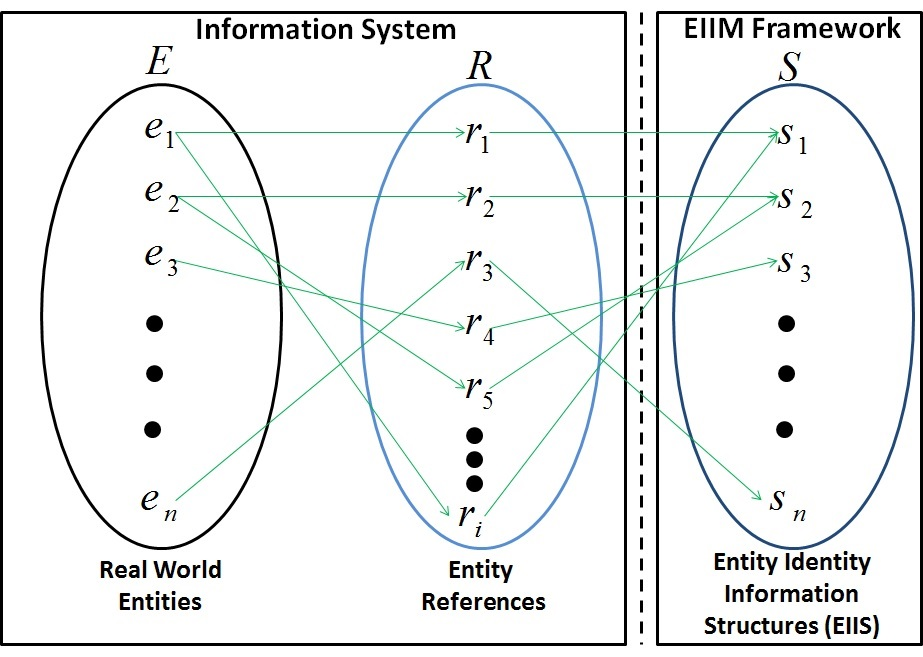
\includegraphics[width=7cm,height=5cm]{Figures/identityIntegrityMDM1.jpg}
\end{figure}



\begin{figure}[htbp]
  \caption{Misjudgments made by EIIM process.}
\label{identityIntegrity2}
  \centering
    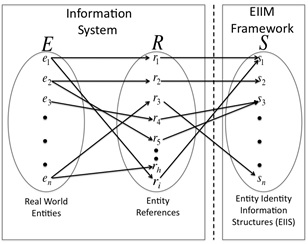
\includegraphics[width=7cm,height=5cm]{Figures/identityIntegrityMDM2.jpg}
\end{figure}


Therefore, ideally in an information system, if $E = \{e_{1},e_{2}, ... ,e_{n}\}$ represents a finite set of entities, $R = \{r_{1},r_{2}, ... ,r_{m}\}$ represents a finite set of references to the entities, and $S = \{s_{1},s_{2}, ... ,s_{n}\}$ represents a finite set of EIIS maintaining identity information of the entities then there should be one-to-one correspondence between the real-life entities ($\in E$) and the EIIS ($\in S$) representing their identity information. Also, the references ($\in R$) of a particular entity ($\in E$) should always map to one and only one EIIS ($\in S$) maintaining its identity information. This is shown in Figure \ref{identityIntegrity1}. Such a situation ensures that the condition of entity identity integrity is satisfied by the information system. One of the main aims of EIIM is to satisfy the conditions of entity identity integrity along with persistently maintaining the entity identity information.

The current EIIM model deals with a closed environment of an information system where there is fixed number of entities along with fixed number of references to them. In an ideal situation the EIIM process should always satisfy the conditions of entity identity integrity as shown in Figure \ref{identityIntegrity1}, and previously explained. However, in practice, all the references to an entity in the information system might not get mapped to the EIIS maintained for that particular entity due to misjudgments made by the automated processes as shown in Figure \ref{identityIntegrity2}. This might result in \textit{false negative} and \textit{false positive} errors. A \textit{false negative} error arises when the system fails to map a reference of an entity to its corresponding EIIS. This is shown in Figure \ref{identityIntegrity2}, where the system fails to map the reference $r_{h}$ ($\in R$) of entity $e_{n}$ ($\in E$) to an EIIS ($\in S$). A \textit{false positive} error arises when the system maps two references of different entities to a single EIIS. This is shown in Figure 5, where the system wrongly maps reference $r_{5}$ ($\in R$) of entity $e_{2}$ ($\in E$), to the EIIS $s_{3}$ ($\in S$) being maintained for entity $e_{3}$ ($\in E$). Such a situation creates dissonance between the actual identity of the real-world entities being stored in the information system and their identities interpreted by the automated processes, resulting in low entity identity integrity of the system. Asserted resolutions are introduced in order to deal with such problems (shown in Figure \ref{originalEIIM}.).

The EIIM processes and life cycle is a step ahead of the basic record linking process that identifies references to same entities for a given dataset. The goal of EIIM is to consistently label references to the same entity with the same identifier across different datasets processed at different times. Through the management of persistent entity identity structures, EIIM provides an added functionality for an entity resolution system to create and assign persistent entity identifiers that do not change from process to process. The current EIIM can also be thought of as forming a nexus between ER and MDM by adding an explicit longitudinal dimension to the management of identity information. The EIIM model proposed in the presented research expands the current model into the unstructured domain of social media, bringing in new challenges and devising new techniques for solving them. The next section gives a detailed discussion and definition of the problem of extending the EIIM model to social media.

\section{Problem of Event Identity Information Management (EIIM) in Social Media\label{problem}}

\begin{figure}[htbp]
  \caption{Event identity information for real-life event, `Egyptian Revolution 2011'.}
\label{eventidentity}
  \centering
    \includegraphics[width=10cm,height=10cm]{Figures/eventIdentity.jpg}
\end{figure}


The definitions as given in the previous section also hold true for the work presented in this dissertation. The only differences are:
\begin{enumerate}
\item We consider a \textbf{real-life event $E_{i}$} as an individual \textbf{entity}, and assume that every \textbf{real-life event} also has a distinct identity. Only a pre-specified set of events $\Xi = \{E_{1},E_{2}, ... ,E_{n}\}$ are considered, with their ordered stream of references $M = \{m_{1_{E_{1}}}, m_{2_{E_{1}}}, ... ,m_{i_{E_{i}}}, ... ,m_{n_{E_{n}}}\}$ collected from social media instead of a fixed set of references already present in a closed information system.

\item Instead of \textbf{Entity Identity Information}, we define \textbf{Event Identity Information} as a set of attributes that distinctly characterizes it and allows that event to be distinguished from all other events maintained by the framework. For example, names of the main active participants (people, organizations, etc), popular keywords, timespan of occurrence and place of occurrence could be identity information for a real-life event as shown in Figure \ref{eventidentity}.

\item Instead of \textbf{Entity Identity Information Structure (EIIS)}, we define \textbf{Event Identity Information Structures (EIIS)}, for real-life events as a data structure that can persistently and efficiently store, retrieve, and manipulate entity identity information. A set of EIIS, $S = \{s_{E_{1}},s_{E_{2}}, ... ,s_{E_{n}}\}$ is maintained, corresponding to each event $E_{i} \in \Xi$ 

\item Lastly, this dissertation solves the problem of \textit{Event Identity Information Management} in the open and unstructured domain of social media, that gives rise to new challenges. It added complexity to the original problem of EIIM, for which following steps are taken (explained in Chapter \ref{eiim}):

\begin{itemize}
\item A completely new life cycle of data processing components had to be introduced that is more suitable for processing unstructured references of events in social media.
\item What consists of \textbf{Event Identity Information} became losely defined due to the unstructured and highly dynamic nature of the environment. This led to development of new techniques that can identify identity information of an event w.r.t time, extract it from the references and store them in the \textbf{Event Identity Information Structures (EIIS)}.
\item A complete new representation of \textbf{Event Identity Information Structures (EIIS)} is proposed, which is more suitable for managing the identity information of events in a dynamic and unstructured environment.
\end{itemize}
\end{enumerate}


%
%
%$R = \{r_{1},r_{2}, ... ,r_{m}\}$
%
%$S = \{s_{1},s_{2}, ... ,s_{n}\}$

\begin{figure}[htbp]
  \caption{Relation between elements of $\Xi,M$ and $S$ in Event Identity Information Management from social media.}
\label{eventresolutionmappings}
  \centering
    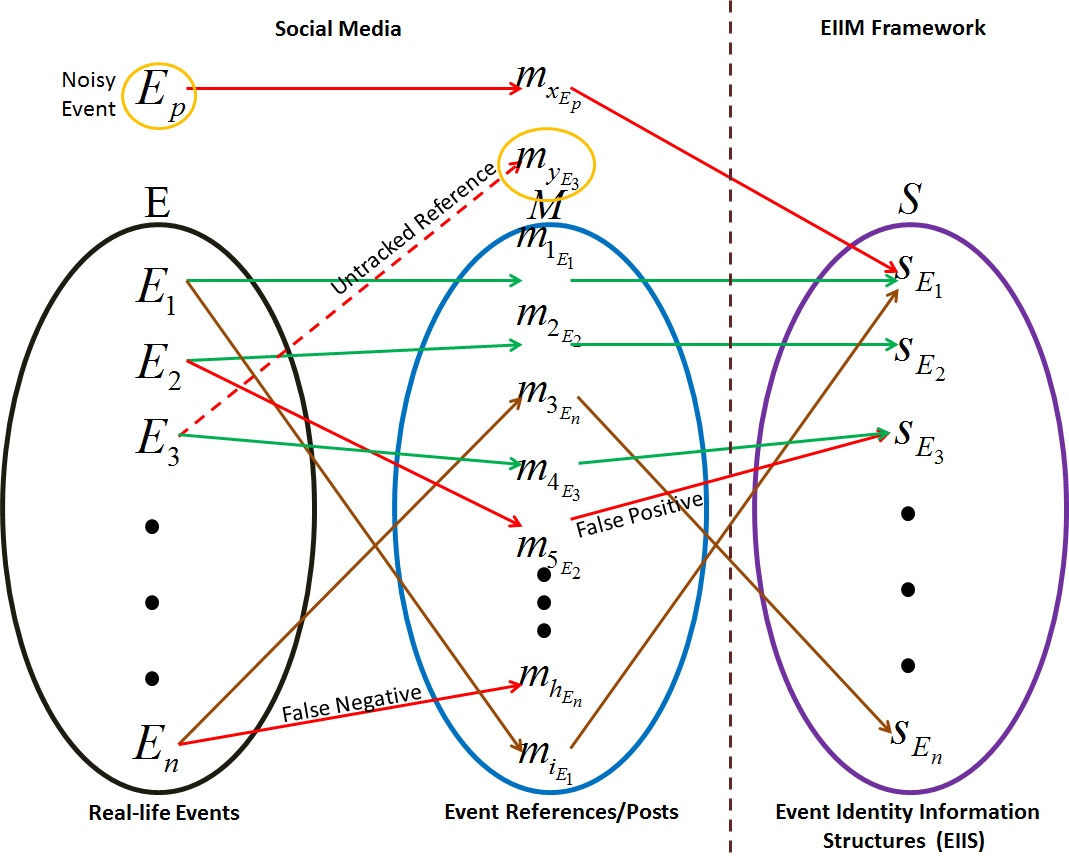
\includegraphics[width=12cm,height=10cm]{Figures/EventResolutionMappings.jpg}
\end{figure}

%In this section, we give the definition of an event appropriate in the context of our problem, and then present a formal statement of the problem that we want to solve.

Events have been defined from various perspectives and in different contexts as already discussed in the previous section. In the context of the work presented in this dissertation we adopt a definition similar to \cite{becker2011beyond}. 


\textbf{Event:} \textit{An event is defined as a real-world occurrence ($ E_{i}$) with an associated time period $T_{E_{i}}$ ($t^{start}_{E_{i}}$-$t^{end}_{E_{i}}$) and a time ordered stream of social media references $M_{E_{i}} = {\{m_{1_{E_{i}}},m_{2_{E_{i}}}, ... ,m_{n_{E_{i}}}, ... ,m_{z_{E_{i}}}\}}$, of substantial volume, discussing about the event and posted in time $T_{E_{i}}$}.

Users in social media post about real-life events in huge volumes and with high velocity. This results in multiple footprints of an event in different social media channels. The footprints could be in the form of textual posts, images, videos or other types of multimedia documents. For example,
following are three different tweets retrieved for the same event ``Sydney Siege Crisis":

\begin{enumerate}
\item RT @cnni: Hostage taker in Sydney cafe demands ISIS flag and call with Australian PM, Sky News reports. http://t.co/a2vgrn30Xh \#sydneysiege
\item ``@carlyeinfeld: Whats with the barking dogs in the background of the briefing on the \#sydneysiege right now?!" Police dogs.
\item @Channel4News The least you could do is to pixelate the faces in the window \#sydneysiege
\end{enumerate}

We consider these footprints as references to the event. One of the main aims of the proposed framework would be to consolidate all the references of a particular event and map it to its corresponding EIIS maintained by the framework. However, due to the noisy nature of social media references an additional problem arise. We call it the problem of noisy reference.

\begin{itemize}
\item \textbf{Noisy Reference:} The three tweets in the example above are different in terms of information content related to the event. While the first one is very informative, the other two are surely related to the event, but not informative. The non-informative tweets might be interesting to the users having a personal conversation related to the event, but it has no value in conveying useful information about the event, that can act as an identity of the event. We consider these event related non-informative references as noise and do not want to map these tweets to the EIIS of the corresponding event. 
\end{itemize}

Also, there might be a mismatch between the way an informative event reference is posted by an user and the way the proposed framework interprets the same in an automated fashion. This would result in loss of data integrity and increase the chances of erroneous results. Such problems are prevalent in the vanilla flavor of the EIIM as discussed in the previous section, giving rise to \textit{false negative} and \textit{false positive} errors. 


Since the Event Identity Information Management framework operates in an open environment of social media as discussed earlier, two new scenarios leading to erroneous conditions are observed:

\begin{itemize}
\item \textbf{Noisy Event} - The first situation occurs when a reference gets mapped to an existing EIIS in the framework, although it refers to an event, which is out of the pre-specified list of events that are being tracked. Such a scenario is shown in Figure \ref{eventresolutionmappings}, where the event $E_{p} \in \Xi$ generates the reference $m_{x_{E_{i}}} \in M_{E_{i}}$, yet the external reference gets mapped to $s_{E_{1}}$. 

Spamming activity in social media channels can give rise to noisy events. For example, if we consider the following tweet:

\begin{itemize}
\item \textit{RT @BFDealz: http://t.co/TSJAigrVJI WHEELS SUPER TREASURE HUNT SUPERIZED HARLEY DAVIDSON FAT BOY LONG CARD 2014 \#cpac2014 \#sxsw}
\end{itemize}

The above tweet might have been posted in the context of the event SXSW 2014 in order to market a Harley Davidson bike, but it also appears in the set of references for an unrelated event CPAC 2014. This is probably due to the fact that both the events took place parallely and the user posting this reference wanted to make it more visible by using the hashtags for both the trending events. This is often the case of spamming activities as discussed in Chapter \ref{challenges}. The tweet might not be related to both the events, yet it can get tracked by the framework.


\item \textbf{Untracked reference} - The second situation occurs when there is a reference, which the framework is unable to track and map it to a pre-specified list of events although it refers to it. Such a scenario is shown in Figure \ref{eventresolutionmappings}, where the framework should have tracked the reference $m_{y_{E_{3}}} \in M_{E_{3}}$ and associate it with event $E_{3} \in \Xi $, yet it is unable to do so and lose track of the reference in the process. This can happen due to the sampling bias as discussed in Chapter \ref{challenges}, which is one of the main challenges in collecting content from social media. The other reason could be errors in data collection process.

\end{itemize}

Therefore, the main broader problem that this dissertation solves is stated below.


\textbf{Problem:} \textit{Given a pre-specified finite set of real-life events, $\Xi = \{E_{1},E_{2}, ... ,E_{n}\}$ generating a finite ordered stream of references $M = \{m_{1_{E_{1}}}, m_{2_{E_{1}}}, ... ,m_{i_{E_{i}}}, ... ,m_{n_{E_{n}}}\}$ in social media, and a finite set of EIIS structures $S = \{s_{E_{1}},s_{E_{2}}, ... ,s_{E_{n}}\}$ corresponding to each real-life event $(E_{i} \in \Xi)$, the problem is to resolve references of an event $(E_{i})$, and to persistently extract, store and manage identity information of the event in its corresponding EIIS $s_{E_{i}}$}.

Towards the above objective, the dissertation seeks answers to the following questions:

\begin{itemize}
\item How to create the set of  EIIS (S) for the pre-specified set of events of interest ?
\item How to collect reference to the events containing identity information of the event from different social media platforms ?
\item How to extract event identity information from the social media references ?
\item How to integrate the event identity information from the unstructured references into the appropriate EIIS ? 
\item How to determine that new references from social media relates to an EIIS ?
\item How to continuously integrate new information into the existing EIIS structures ?


\end{itemize}

Chapter \ref{eiim} presents the design and implementation of the entire Event Identity Information Management framework that explains the strategies and novel techniques contributed by this dissertation in order to find answers to the above questions. A detailed survey of the existing literature related to the problem is presented in the next Chapter.



%The tweets are primarily composed of a set of hashtags ($\scriptstyle H_{E_{i}}$) used for annotating the tweets ($\scriptstyle \in M_{E_{i}}$), a set of text units ($\scriptstyle W_{E_{i}}$) used for sharing textual information in the tweets ($\scriptstyle \in M_{E_{i}}$), a set of URLs ($\scriptstyle L_{E_{i}}$) linking to external sources related to the event and a  set of users ($\scriptstyle U_{E_{i}}$) posting the tweets ($\scriptstyle \in M_{E_{i}}$).
%\item a set of hashtags ($H_{E_{i}}$) used for annotating the tweets ($\in M_{E_{i}}$) related to the event.
%\item a set of users ($U_{E_{i}}$) posting tweets ($\in M_{E_{i}}$) about the event.
%\item a set of urls ($L_{E_{i}}$) linking to external sources related to the event, shared by the users ($\in U_{E_{i}}$) in the tweets ($\in M_{E_{i}}$) posted by them.
%\item a set of text units ($W_{E_{i}}$) used for sharing textual information in the tweets ($\in M_{E_{i}}$) about the event.

